\section{Aufbau und Durchführung}
\label{sec:Durchführung}

    \noindent In dem Versuch soll die Aktivierungsenergie und die Relaxationszeit von Dipolen in dotierten Ionenkristallen ermittelt werden. 
    Der Aufbau ist in der \autoref{fig:aufbau} zu sehen. 
    \begin{figure}[h]
        \centering
        %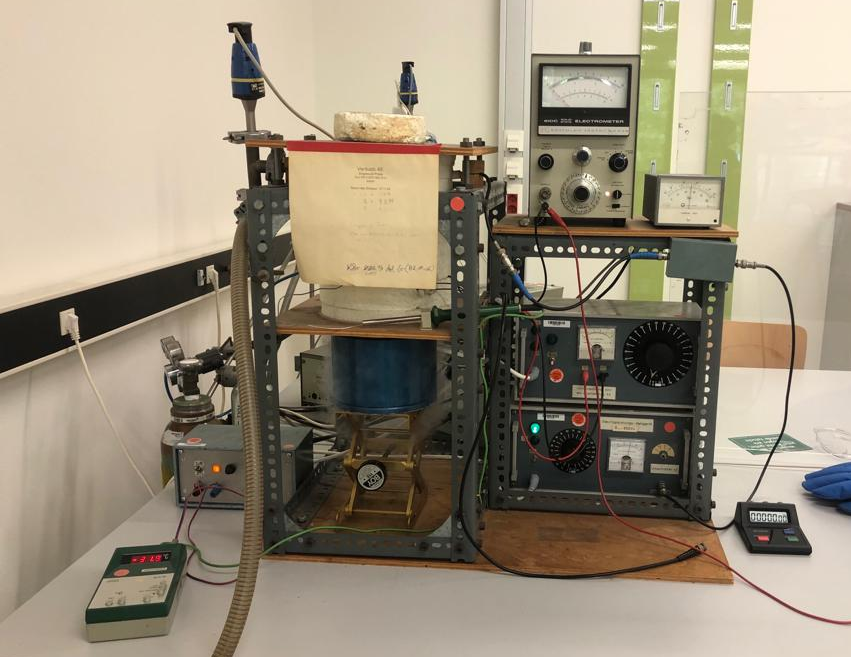
\includegraphics[width=0.7\textwidth]{bilder/foto_aufbau.png}
        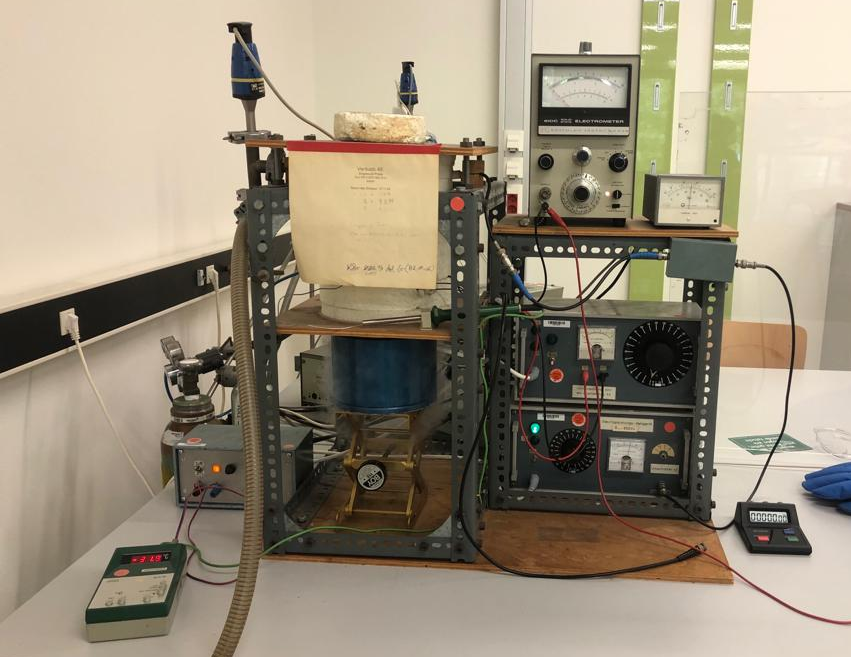
\includegraphics[width=\textwidth]{bilder/foto_aufbau.png}
        \caption{Die Messapparatur, wie sie im Versuch benutzt wird. \cite{anleitung}}
        \label{fig:aufbau}
    \end{figure}
    Die zu untersuchende Probe ist in dem mit Styropor ummantelten Zylinder zu finden. Die Kondensatorplatten sind am oberen und am unteren Ende des Zylinders 
    angebracht. Die Hochspannung wird mit dem unteren Generator auf der rechten Seite eingestellt. Die untere Kondensatorplatte ist mit dem Heizgerät verbunden, welche über den 
    oberen Generator eingestellt wird. In dem Foto wird die Probe durch flüssigen Stickstoff gekühlt. Dieser befindet sich in dem Dewargefäß unter dem Zylinder, wobei 
    in diesen ein Kühlfinger taucht. Die Temperatur ist auf dem grünen Messgerät abzulesen. Der dicke Schlauch führt von der Drehschieber-Vakuumpumpe 
    zum Zylinder. Auf der rechten Seite steht oben ein Picoamperemeter und ein Manometer, welches den Druck des Vakuums an der Probe misst. 
    Die Handschuh auf der rechten Seite werden dafür benutzt das Dewargefäß mit flüssigem Stickstoff zu befühlen. 

    \noindent Um die Eigenschaften von Dipolen in Ionenkristallen zu ermitteln, muss der Depolarisationsstrom bei einer gewissen Temperatur kontrolliert 
    gemessen werden. Dafür wird der Kristall zuerst erwärmt auf eine Temperatur von $\SI{50}{\celsius} / \SI{323.15}{\kelvin}$, während ein Vakuum von etwa $\SI{e-2}{\milli\bar}$ aufrecht gehalten werden soll, da 
    die Kristalle hygroskopisch sind und sich sonst sehr viele Wasserdipole ausbilden, die einen größeren Untergrund in der Messung darstellen. 
    Bei der Erwärmung des Kristalles wird das elektrische Feld mittels des Plattenkondensators an einer Spannung von $\SI{900}{\volt}$ aufgebaut. Dadurch werden die Dipole entlang des elektrischen 
    Feldes ausgerichtet. Das elektrische Feld wird aufrechtgehalten und die Probe mit flüssigen Stickstoff gekühlt, sodass die Ausrichtung der Dipole 
    beibehalten wird. Bei einer Temperatur von etwa $\SI{-60}{\celsius}/ \SI{213.15}{\kelvin}$ ist die Relaxationszeit so groß, dass der Kondensator abgeschalten wird 
    und die gesamte Ladung innerhalb von $\SI{5}{\minute}$ vom Kondensator abgefliessen soll. Nachdem der Kondensator entladen ist, wird das Picoamperemeter 
    angeschlossen und die Messung angefangen. Mit dem Heizgerät soll eine konstante Heizrate eingestellt werden, $\SI{1.5}{\kelvin\per\minute}$ oder $\SI{2}{\kelvin\per\minute}$, 
    und dann wird jede Minute die Temperatur und der Strom gemessen und aufgeschrieben. Der Ionenkristall hat einen Gesamtdipolmoment, da die Dipole 
    gleich ausgerichtet sind. Orientiert sich ein Dipol um, da er die Aktivierungsenergie $W$ aufbringen kann, verändert sich das Gesamtdipolmoment 
    und somit auch das elektrische Feld, welches vom Kristall ausgeht. Da das komplette elektrische Feld zwischen den Platten des Kondensator gleich bleiben soll, 
    muss ein Strom fließen. Die Messung wird bei einer Temperatur von $\SI{60}{\celsius}/ \SI{333.15}{\kelvin}$ 
    abgeschlossen. 
